\documentclass[10pt,aspectratio=169]{beamer}
\usetheme[progressbar=frametitle,numbering=fraction]{metropolis}
\usepackage[T1]{fontenc}
\usepackage[utf8]{inputenc}
\usepackage[italian]{babel}
\usepackage{lmodern}
\usepackage{amsmath,amssymb,mathtools}
% Simbolo corretto per la funzione indicatrice (1 a doppio tratto).
\usepackage{dsfont}
\usepackage{booktabs,tabularx,array,multirow}
\usepackage{tikz}
\usetikzlibrary{arrows.meta,positioning,calc,shapes.geometric}
\usepackage{graphicx}
\usepackage[table]{xcolor}
\usepackage{ragged2e}
\usepackage{microtype}
\graphicspath{{assets/}}
\definecolor{deepnavy}{HTML}{152B42}
\definecolor{teal}{HTML}{007D88}
\definecolor{pale}{HTML}{EAF2F3}
\definecolor{orange}{HTML}{D08035}
\definecolor{softgray}{HTML}{607181}
\definecolor{mygreen}{HTML}{21655E}
\setbeamercolor{normal text}{fg=deepnavy,bg=white}
\setbeamercolor{frametitle}{fg=white,bg=deepnavy}
\setbeamercolor{title}{fg=deepnavy}
\setbeamercolor{subtitle}{fg=softgray}
\setbeamercolor{progress bar}{fg=teal,bg=pale}
\setbeamercolor{alerted text}{fg=teal}
\setbeamercolor{block title}{fg=deepnavy,bg=pale}
\setbeamercolor{block body}{fg=deepnavy,bg=pale}
\setbeamerfont{frametitle}{size=\large,series=\bfseries}
\setbeamerfont{title}{size=\LARGE,series=\bfseries}
\setbeamerfont{subtitle}{size=\normalsize}
\setbeamertemplate{navigation symbols}{}
\setbeamertemplate{itemize item}{\color{teal}$\blacktriangleright$}
\setbeamertemplate{itemize subitem}{\color{teal}$\bullet$}
\setlength{\tabcolsep}{6pt}
\renewcommand{\arraystretch}{1.19}
\newcommand{\source}[1]{\par\vspace{2pt}{\tiny\color{softgray}#1}}
\newcommand{\keypoint}[1]{\par\vspace{0.45em}\noindent{\color{teal}\rule{2.4pt}{1.25em}}\hspace{0.7em}\parbox[t]{0.92\linewidth}{\raggedright\textbf{#1}}}
\newcommand{\tightitems}{\setlength{\itemsep}{.5em}}
\newcommand{\scorenote}[2]{\begin{minipage}{.47\linewidth}\centering{\Large\bfseries\color{teal}#1}\\[-.1em]{\small #2}\end{minipage}}
\title{Predicting Term Deposit Subscription}
\subtitle{Bank Marketing: un approccio di classificazione supervisionata}
\author{Davide De Santis}
\date{Progetto di Machine Learning \;|\; A.A. 2025--2026}
\titlegraphic{}
\begin{document}

\begin{frame}[plain]
\vspace*{.55cm}
{\LARGE\bfseries\color{deepnavy}Predicting Term Deposit Subscription}\par\vspace{.45em}
{\large\color{softgray}Bank Marketing: un approccio di classificazione supervisionata}\par\vspace{1.0cm}
{\color{teal}\rule{.91\linewidth}{1.2pt}}\par
\vfill
{\normalsize\bfseries Davide De Santis}\par\vspace{.24em}
{\small Progetto di Machine Learning\quad A.A. 2025--2026}\par\vspace{.5cm}
\end{frame}

\begin{frame}{Obiettivo: identificare i clienti prioritari}
\begin{columns}[T,onlytextwidth]
\column{.58\textwidth}
\textbf{Scenario operativo}\par\medskip
Prima che il prossimo contatto telefonico venga programmato o effettuato, assegnare a ogni cliente uno \alert{score di propensione} alla sottoscrizione di un deposito a termine.
\vspace{1em}
\begin{itemize}\tightitems
\item Problema di \textbf{classificazione binaria}: $Y\in\{0,1\}$.
\item Quantità teorica: $P(Y=1\mid X=x)$.
\item Output del modello: $\hat p(x)$, utilizzato per \textbf{ranking} e classificazione.
\end{itemize}
\column{.38\textwidth}
\begin{block}{Regola decisionale}
\vspace{-.6em}
\[\hat y=\begin{cases}1&\hat p(x)\geq\tau\\0&\hat p(x)<\tau\end{cases}\]
\vspace{-.5em}
\end{block}
\vspace{.8em}
{\small La soglia $\tau$ sarà scelta \emph{dopo} il confronto dei modelli.}
\end{columns}
\end{frame}

\begin{frame}{Dataset: UCI Bank Marketing}
\begin{columns}[T,onlytextwidth]
\column{.43\textwidth}
\begin{tabular}{@{}lr@{}}\toprule
Osservazioni & \textbf{45.211}\\
Predittori originali & \textbf{16}\\
Target & \textbf{1}\\
Task & \textbf{Binario}\\\bottomrule\end{tabular}
\vspace{1em}
\begin{itemize}\tightitems
\item Variabili numeriche e categoriche.
\item Nessun valore NaN rilevato.
\item La categoria \texttt{unknown} è mantenuta come modalità valida.
\end{itemize}
\column{.54\textwidth}
\textbf{Gruppi di variabili}\par\smallskip
\begin{tabular}{@{}p{.28\linewidth}p{.65\linewidth}@{}}\toprule
Profilo & \texttt{age}, \texttt{job}, \texttt{education}, \texttt{balance}, \texttt{housing}, \texttt{loan}, \dots\\
Contatti & \texttt{campaign}, \texttt{day}, \texttt{month}, \texttt{contact}, \texttt{duration}\\
Storico & \texttt{pdays}, \texttt{previous}, \texttt{poutcome}\\\bottomrule\end{tabular}
\end{columns}
\source{Fonte: UCI Bank Marketing, file \texttt{bank-full.csv} (recuperato dal mirror Kaggle indicato nel notebook).}
\end{frame}

\begin{frame}{Prediction setting e disponibilità delle informazioni}
\begin{columns}[T,onlytextwidth]
\column{.51\textwidth}
\textbf{Feature escluse dal modello principale}
\vspace{.45em}
\begin{tabular}{@{}ll@{}}\toprule
\texttt{contact} & Canale del contatto\\
\texttt{day}, \texttt{month} & Data del contatto\\
\texttt{duration} & Durata della chiamata\\\bottomrule\end{tabular}
\par\vspace{.75em}
{\small\noindent\parbox{\linewidth}{Nello scenario scelto queste variabili non vengono considerate disponibili al momento della previsione.}}
\column{.46\textwidth}
\begin{block}{Scelta centrale del progetto}
Una feature molto predittiva non è necessariamente \textbf{utilizzabile al prediction time}.
\end{block}
\vspace{.8em}
{\small L'esclusione è un'\textbf{assunzione operativa} del progetto, non una proprietà universale del dataset.}
\end{columns}
\end{frame}

\begin{frame}{Protocollo sperimentale: separare selezione e valutazione}
\centering
\begin{tikzpicture}[every node/.style={font=\small}, box/.style={draw=deepnavy!25,rounded corners=2pt,fill=pale,minimum height=8mm,align=center}, arr/.style={-Latex,thick,draw=teal}]
\node[box,minimum width=35mm] (d) at (0,0) {Dataset\\45.211 osservazioni};
\node[box,minimum width=38mm] (tr) at (-3,-1.25) {Training (80\%)\\36.168};
\node[box,minimum width=38mm] (ts) at (3,-1.25) {Test (20\%)\\9.043};
\node[box,minimum width=47mm] (cv) at (-3,-2.5) {5-fold stratified CV\\modelli, tuning, PCA, selection};
\node[box,minimum width=47mm] (tau) at (-3,-3.75) {OOF predictions\\scelta soglia $\tau$};
\node[box,minimum width=38mm] (fin) at (3,-3.25) {Valutazione finale\\a scelte fissate};
\draw[arr] (d)--(tr);\draw[arr] (d)--(ts);\draw[arr] (tr)--(cv);\draw[arr] (cv)--(tau);\draw[arr] (ts)--(fin);
\end{tikzpicture}
\par\vspace{.15em}
{\footnotesize Split stratificato sul target, \texttt{random\_state=42}; preprocessing rifittato dentro ogni fold.}
\end{frame}

\begin{frame}{Class imbalance: perché non ottimizzare l'Accuracy?}
\begin{columns}[c,onlytextwidth]
\column{.55\textwidth}
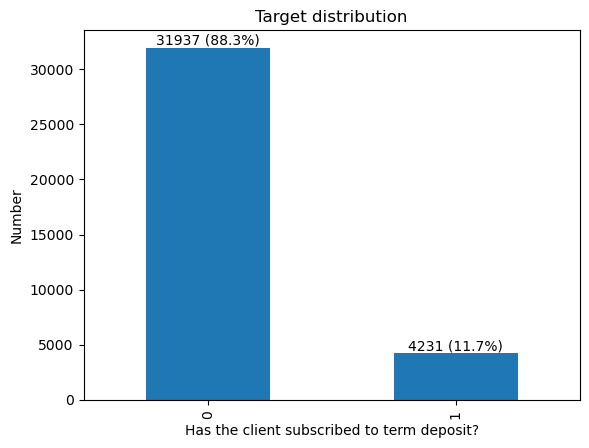
\includegraphics[width=\linewidth,height=.65\textheight,keepaspectratio]{plot_cell_12_1.png}
\column{.42\textwidth}
\scorenote{11,7\%}{classe positiva}\par\vspace{1.3em}
\scorenote{88,3\%}{accuracy del classificatore sempre negativo}\par\vspace{1.1em}
{\small Una buona Accuracy non implica il riconoscimento dei clienti che sottoscrivono.}
\end{columns}
\end{frame}

\begin{frame}{Metrica primaria: Average Precision}
\begin{columns}[T,onlytextwidth]
\column{.58\textwidth}
\textbf{Average Precision (AP)} sintetizza la curva Precision--Recall al variare della soglia:
\[\mathrm{AP}=\sum_k (R_k-R_{k-1})P_k\]
\begin{itemize}\tightitems
\item Valuta la qualità del \textbf{ranking degli esempi positivi}.
\item Evita di fissare subito un threshold.
\item È più informativa dell'Accuracy per l'obiettivo del progetto.
\end{itemize}
\column{.37\textwidth}
\begin{block}{Punto di riferimento}
\centering
{\LARGE\bfseries\color{teal} AP $\approx$ 0,117}
\par\smallskip
{\small Ranking non informativo, con prevalenza positiva $\approx 11,7\%$.}
\end{block}
\vspace{.5em}
{\footnotesize Precision, Recall, F1 e ROC-AUC rimangono metriche complementari.}
\end{columns}
\end{frame}

\section{Exploratory Data Analysis}

\begin{frame}{EDA: associazioni marginali con il target}
\begin{columns}[c,onlytextwidth]
\column{.58\textwidth}
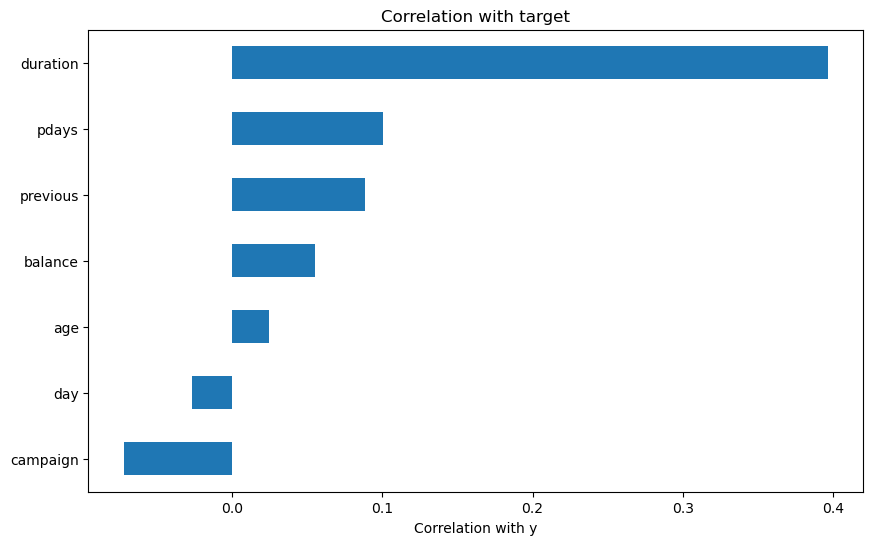
\includegraphics[width=\linewidth,height=.72\textheight,keepaspectratio]{plot_cell_16_1.png}
\column{.39\textwidth}
\textbf{Osservazioni}\vspace{.4em}
\begin{itemize}\tightitems
\item \texttt{duration}: associazione numerica più marcata.
\item \texttt{pdays}, \texttt{previous}, \texttt{balance}: correlazione positiva.
\item \texttt{campaign}: correlazione negativa.
\end{itemize}
\smallskip
{\small Analisi \textbf{esplorativa} sul solo training: correlazione $\neq$ causalità.}
\end{columns}
\end{frame}

\begin{frame}{EDA: distribuzione di \texttt{balance}}
\centering
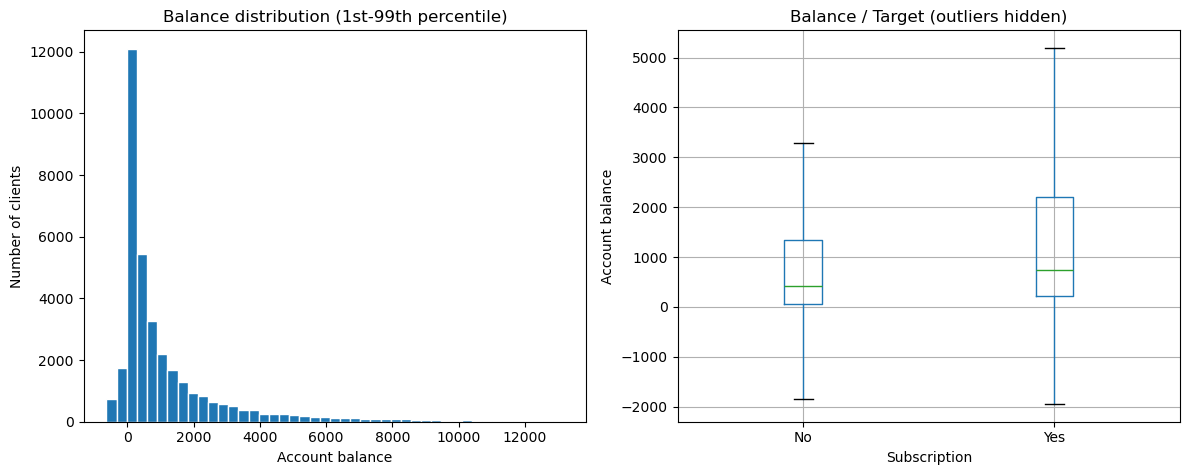
\includegraphics[width=.94\linewidth,height=.66\textheight,keepaspectratio]{plot_cell_20_0.png}
\par\vspace{.25em}
\raggedright\small
Mediana $\approx740$ euro per $Y=1$ e $\approx419$ euro per $Y=0$; distribuzione fortemente asimmetrica. Il taglio dei percentili è usato solo per la visualizzazione.
\end{frame}

\begin{frame}{EDA: distribuzione di \texttt{age}}
\centering
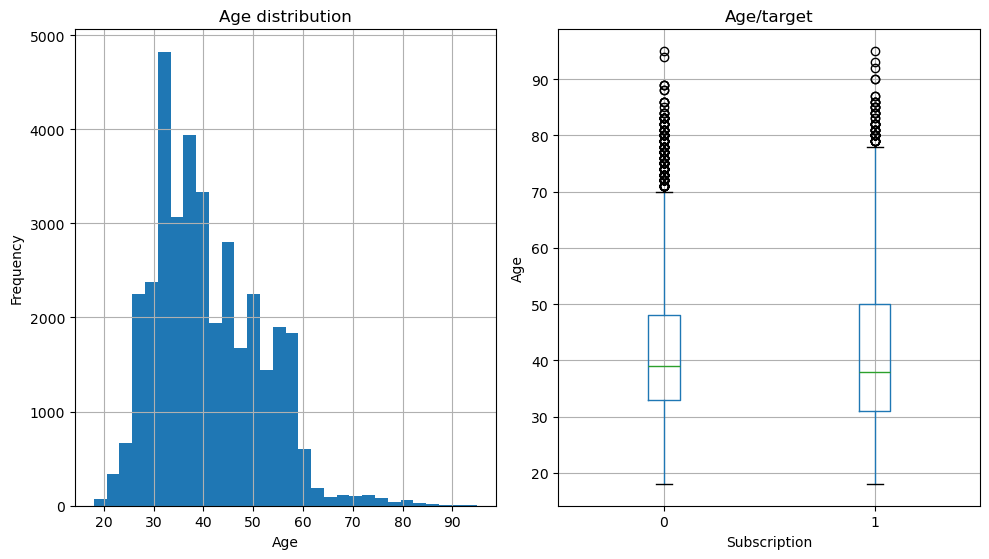
\includegraphics[width=.88\linewidth,height=.65\textheight,keepaspectratio]{notebook_cell_17_img_0.png}
\par\vspace{.30em}
\raggedright\small
Età media $\approx41,6$ anni per $Y=1$ e $\approx40,8$ per $Y=0$: le distribuzioni si sovrappongono ampiamente. La feature, considerata da sola, ha potere discriminativo limitato.
\end{frame}

\begin{frame}{EDA: contatti durante la campagna}
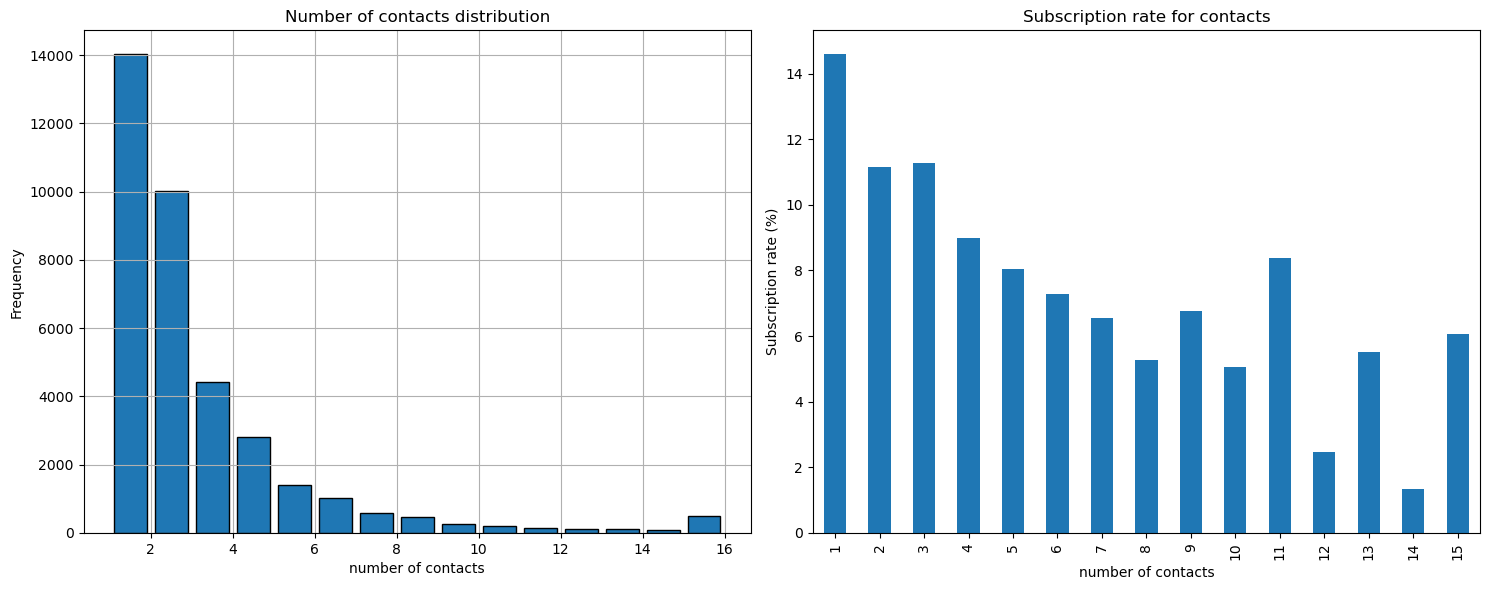
\includegraphics[width=.88\linewidth,height=.65\textheight,keepaspectratio]{plot_cell_22_0.png}
\vspace{.1em}
\keypoint{\texttt{campaign} è asimmetrica: più contatti osservati si associano generalmente a un minor tasso di sottoscrizione.}
\source{Associazione descrittiva, non interpretata causalmente; support più piccolo per conteggi elevati.}
\end{frame}

\begin{frame}{EDA: storia dei contatti precedenti}
\begin{columns}[c,onlytextwidth]
\column{.47\textwidth}
\textbf{Il valore speciale di \texttt{pdays}}\vspace{.6em}
\begin{tabular}{@{}lr@{}}\toprule
Storia precedente & Tasso $Y=1$\\\midrule
Mai contattato ($-1$) & \textbf{9,2\%}\\
Già contattato & \textbf{22,8\%}\\\bottomrule\end{tabular}
\vspace{.9em}
\textbf{Interpretazione}: l'assenza di storia non è semplicemente una distanza temporale.
\column{.50\textwidth}
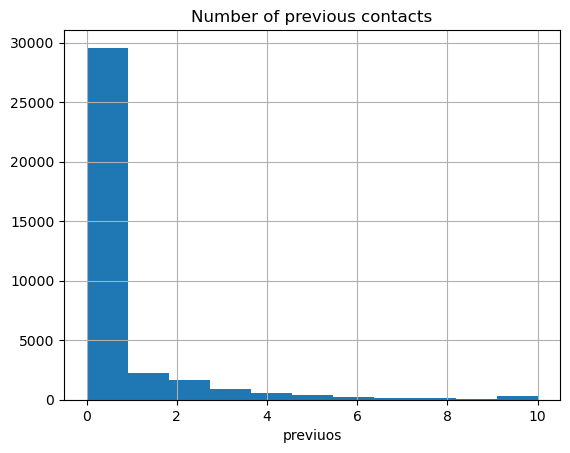
\includegraphics[width=\linewidth,height=.59\textheight,keepaspectratio]{plot_cell_26_0.png}
{\footnotesize \texttt{previous}: distribuzione concentrata in zero.}
\end{columns}
\end{frame}

\begin{frame}{EDA: profilo del cliente -- \texttt{job}}
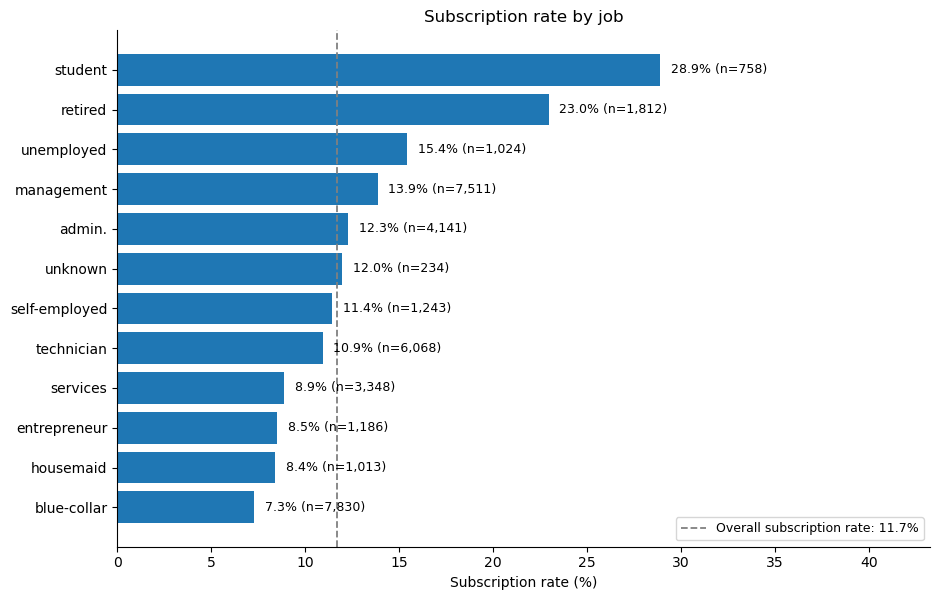
\includegraphics[width=.88\linewidth,height=.66\textheight,keepaspectratio]{plot_cell_29_0.png}
\keypoint{Studenti e pensionati hanno tassi di sottoscrizione relativamente elevati; per ogni categoria va considerato anche il support.}
\end{frame}

\begin{frame}{EDA: istruzione e mutuo immobiliare}
\begin{columns}[c,onlytextwidth]
\column{.50\textwidth}
\textbf{\texttt{education}}\par\smallskip
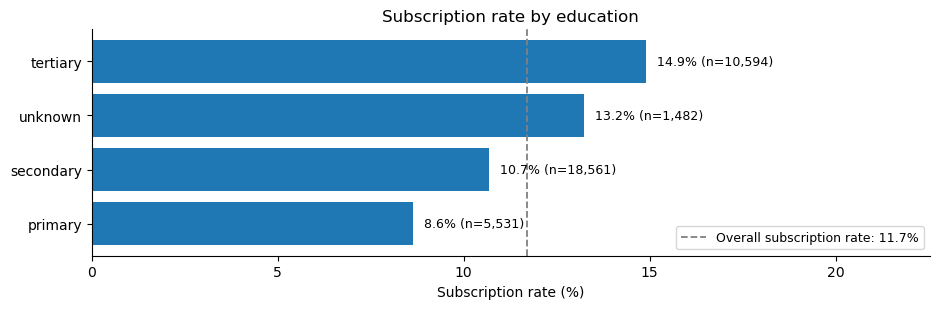
\includegraphics[width=\linewidth,height=.45\textheight,keepaspectratio]{plot_cell_30_0.png}
\column{.49\textwidth}
\textbf{\texttt{housing}}\par\smallskip
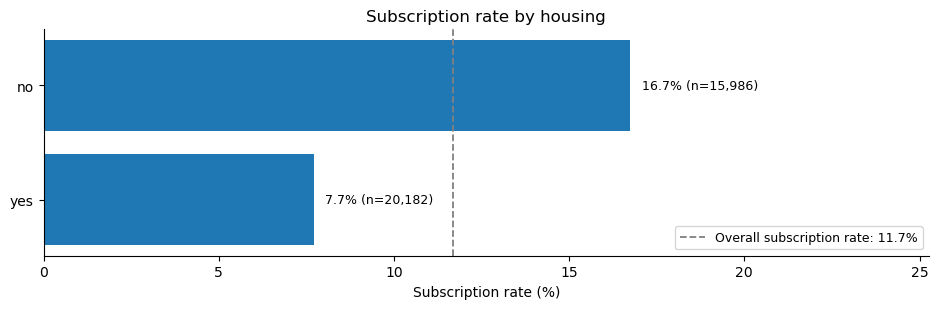
\includegraphics[width=\linewidth,height=.45\textheight,keepaspectratio]{plot_cell_32_0.png}
\end{columns}
\keypoint{I tassi variano con le caratteristiche socio-economiche, ma nessuna feature marginale risolve da sola il problema.}
\end{frame}

\begin{frame}{EDA: prestito personale e campagna precedente}
\begin{columns}[T,onlytextwidth]
\column{.49\textwidth}
\textbf{\texttt{loan}}\par\smallskip
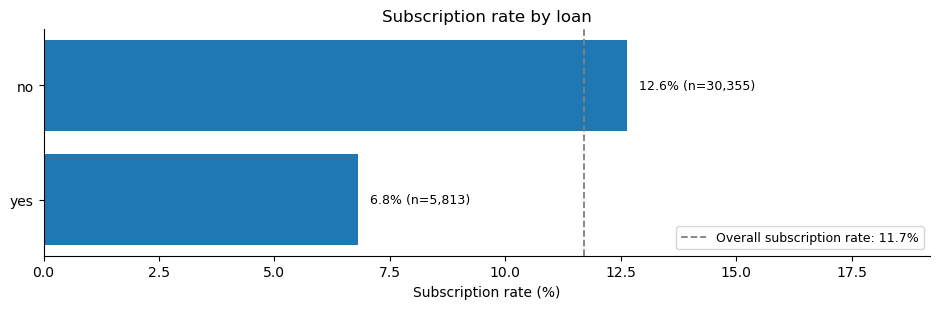
\includegraphics[width=\linewidth,height=.47\textheight,keepaspectratio]{plot_cell_33_0.png}
\column{.49\textwidth}
\textbf{\texttt{poutcome}}\par\smallskip
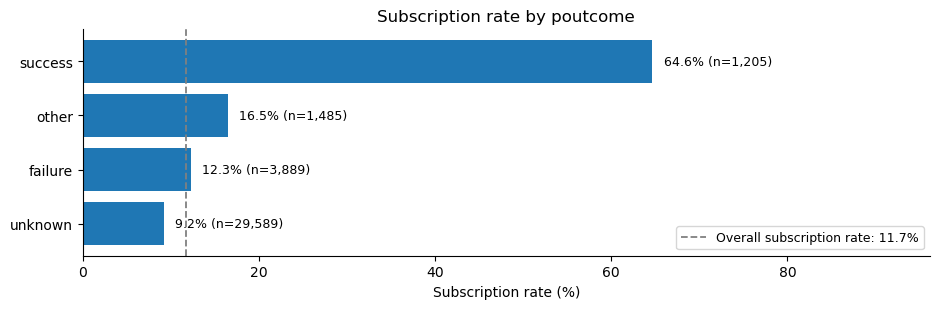
\includegraphics[width=\linewidth,height=.47\textheight,keepaspectratio]{plot_cell_35_0.png}
\end{columns}
\vspace{-.3em}
\keypoint{\texttt{poutcome=success} è fortemente associata alla sottoscrizione nella campagna osservata.}
\end{frame}

\begin{frame}{EDA: feature informative ma non utilizzabili}
\begin{columns}[c,onlytextwidth]
\column{.45\textwidth}
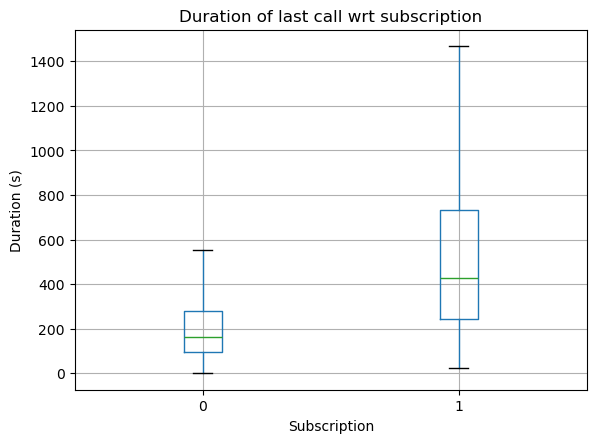
\includegraphics[width=\linewidth,height=.57\textheight,keepaspectratio]{plot_cell_38_1.png}
{\footnotesize Durata della chiamata distinta per classe.}
\column{.51\textwidth}
\begin{itemize}\tightitems
\item La \texttt{duration} risulta particolarmente associata al target.
\item È nota \textbf{solo dopo il contatto}.
\item La sua inclusione viene valutata \emph{separatamente} come esperimento diagnostico.
\end{itemize}
\end{columns}
\end{frame}

\section{Modelli e validazione}

\begin{frame}{Feature engineering: una rappresentazione coerente}
\begin{enumerate}\setlength{\itemsep}{1em}
\item \textbf{Eliminazione delle feature assunte non disponibili}: \texttt{contact}, \texttt{day}, \texttt{month}, \texttt{duration}.
\item \textbf{Storia dei contatti}: codifica esplicita del valore speciale
\[\mathrm{prev\_cont}=\mathds{1}_{\{\mathrm{pdays}\neq -1\}}.\]
\item \textbf{Numero di contatti precedenti nella campagna}:
\[\mathrm{log\_campaign}=\log(1+\mathrm{campaign}-1)=\log(\mathrm{campaign}).\]
\end{enumerate}
\vspace{-.6em}
\source{La ricostruzione di \texttt{campaign}-1 si basa sul prediction setting adottato.}
\end{frame}

\begin{frame}{Preprocessing senza leakage tra fold}
\begin{columns}[T,onlytextwidth]
\column{.48\textwidth}
\begin{block}{Numeriche}
\centering \texttt{StandardScaler}
\end{block}
\begin{block}{Categoriche}
\centering {\footnotesize\texttt{OneHotEncoder(handle\_unknown="ignore")}}
\end{block}
\column{.49\textwidth}
\begin{block}{Integrazione}
\centering \texttt{ColumnTransformer}\\\medskip
\texttt{Pipeline}\\\medskip
\texttt{StratifiedKFold(5)}
\end{block}
\end{columns}
\vspace{.6em}
\centering\textbf{35 colonne trasformate} (numeriche + indicatori one-hot).\par
\vspace{.45em}
{\small Scaling, encoding e successivamente eventuale selezione/PCA vengono appresi solo sul training fold.}
\end{frame}

\begin{frame}{Modelli: confronto tra ipotesi induttive}
\small
\begin{tabularx}{\linewidth}{@{}p{.24\linewidth}X X@{}}\toprule
\textbf{Modello} & \textbf{Caratteristica} & \textbf{Motivazione nel progetto}\\\midrule
Logistic Regression & Modello lineare probabilistico & Riferimento semplice e interpretabile\\
Linear SVC & Modello lineare basato sul margine & Confronto con diversa funzione obiettivo\\
Decision Tree & Split gerarchici non lineari & Interazioni e strutture non lineari\\
Random Forest & Ensemble di alberi & Verificare i benefici dell'aggregazione e del tuning\\
DummyClassifier & Classe maggioritaria & Baseline non predittiva\\\bottomrule\end{tabularx}
\vspace{.7em}
\keypoint{Si confrontano approcci lineari, non lineari ed ensemble.}
\end{frame}

\begin{frame}{Primo confronto: 5-fold stratified CV}
\centering
\begin{tabular}{@{}lrr@{}}\toprule
\textbf{Modello} & \textbf{AP media} & \textbf{Dev. std.}\\\midrule
Dummy baseline & 0,1170 & 0,0001\\
Logistic Regression & \textbf{0,3550} & 0,0106\\
Logistic Regression balanced & 0,3525 & 0,0102\\
Decision Tree & 0,3114 & 0,0223\\
Random Forest & 0,3219 & 0,0153\\
Linear SVC & 0,3511 & 0,0099\\\bottomrule
\end{tabular}
\vspace{1em}
\keypoint{Le tre famiglie più promettenti per AP: Logistic Regression, Linear SVC e Random Forest.}
\end{frame}

\begin{frame}{Imbalance: effetto di \texttt{class\_weight=balanced}}
\begin{columns}[T,onlytextwidth]
\column{.62\textwidth}
\begin{tabular}{@{}lrr@{}}\toprule
\textbf{Metrica} & \textbf{Logistic} & \textbf{Balanced}\\\midrule
Precision & 0,666 & 0,229\\
Recall & 0,162 & 0,597\\
F1 & 0,261 & 0,331\\
AP & 0,355 & 0,353\\\bottomrule\end{tabular}
\column{.34\textwidth}
\begin{block}{Osservazione}
La pesatura modifica molto il \textbf{punto operativo}, ma non migliora l'AP.
\end{block}
\end{columns}
\vspace{1em}
{\small La metrica di ranking e le metriche ottenute con una soglia fissata descrivono aspetti differenti.}
\end{frame}

\begin{frame}{Hyperparameter tuning: impostazione}
\begin{columns}[T,onlytextwidth]
\column{.49\textwidth}
\textbf{Logistic Regression / Linear SVC}
\begin{itemize}\tightitems
\item $C\in\{0.01,0.1,1,10,100\}$
\item \texttt{class\_weight} $\in\{$\texttt{None}, \texttt{balanced}$\}$
\end{itemize}
\vspace{.6em}
\textbf{Strumento}: \texttt{GridSearchCV}\par
\textbf{Metrica}: Average Precision
\column{.49\textwidth}
\textbf{Random Forest}
\begin{itemize}\tightitems
\item \texttt{n\_estimators} $\in\{100,300\}$
\item \texttt{max\_depth} $\in\{\mathrm{None},5,10\}$
\item \texttt{min\_samples\_leaf} $\in\{1,5,10\}$
\item \texttt{class\_weight} $\in\{$\texttt{None}, \texttt{balanced}$\}$
\end{itemize}
\end{columns}
\vspace{.45em}
\keypoint{Ogni configurazione include nuovamente il preprocessing nella CV.}
\end{frame}

\begin{frame}{Hyperparameter tuning: i modelli selezionati}
\centering
\begin{tabular}{@{}lrr@{}}\toprule
\textbf{Modello} & \textbf{CV AP} & \textbf{Dev. std.}\\\midrule
Logistic Regression ($C=1$) & 0,3550 & 0,0106\\
Linear SVC ($C=0.01$) & 0,3518 & 0,0094\\
\rowcolor{pale} Random Forest & \textbf{0,3841} & 0,0144\\\bottomrule\end{tabular}
\vspace{.85em}
\begin{block}{Random Forest: migliore configurazione}
\centering\texttt{n\_estimators=300} \; $\mid$ \; \texttt{max\_depth=10}\\
\texttt{min\_samples\_leaf=10} \; $\mid$ \; \texttt{class\_weight=None}
\end{block}
\keypoint{La Random Forest ottimizzata supera la Logistic Regression di circa 0,029 punti di AP.}
\end{frame}

\begin{frame}{Stabilità del confronto nei cinque fold}
\begin{columns}[c,onlytextwidth]
\column{.69\textwidth}
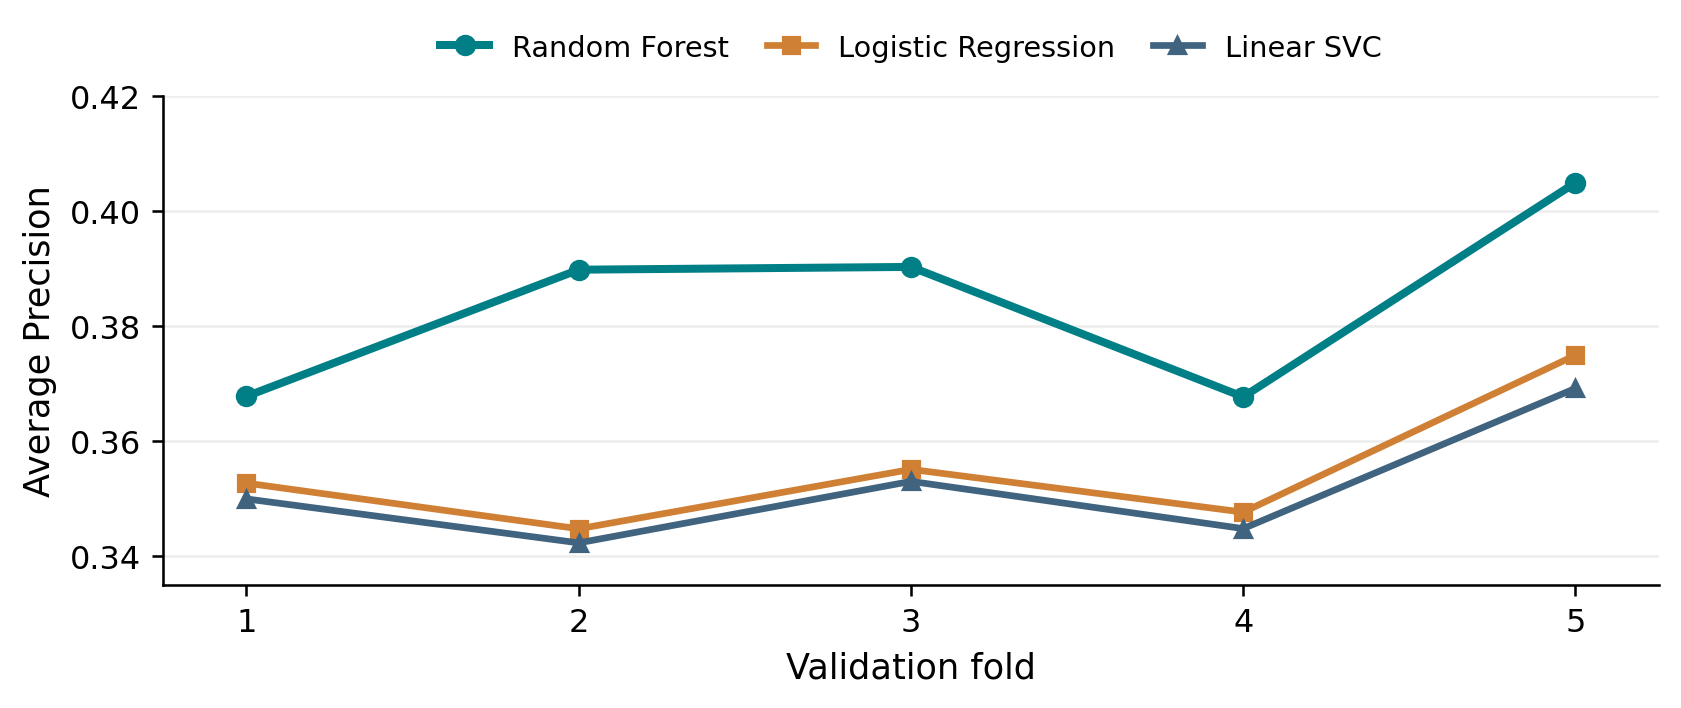
\includegraphics[width=\linewidth,height=.67\textheight,keepaspectratio]{fold_ap_clean.png}
\column{.28\textwidth}
\textbf{Osservazione}\par\medskip
La Random Forest ottimizzata ottiene AP più elevata sia della Logistic Regression sia della SVC in tutti i cinque validation fold.
\end{columns}
\end{frame}

\begin{frame}{Overfitting: prima e dopo il tuning}
\centering
\begin{tabular}{@{}lrrr@{}}\toprule
\textbf{Random Forest} & \textbf{Train AP} & \textbf{Val. AP} & \textbf{Gap}\\\midrule
Iniziale & 0,9999 & 0,3219 & 0,6780\\
\rowcolor{pale} Ottimizzata & 0,4479 & \textbf{0,3841} & \textbf{0,0638}\\\bottomrule\end{tabular}
\vspace{1.2em}
\begin{columns}[T,onlytextwidth]
\column{.48\textwidth}
\textbf{Iniziale}: quasi perfetta sui training fold ma molto peggiore sui validation fold.
\column{.48\textwidth}
\textbf{Ottimizzata}: alberi meno complessi, minore gap, maggiore validation AP.
\end{columns}
\vspace{1em}
\keypoint{Evidenza forte di overfitting iniziale e riduzione del gap dopo il tuning.}
\end{frame}

\section{Riduzione della dimensionalità}

\begin{frame}{Feature selection: Logistic Regression e penalità $L^1$}
\begin{columns}[T,onlytextwidth]
\column{.51\textwidth}
\textbf{Metodo}\par\medskip
\texttt{SelectFromModel} con Logistic Regression penalizzata $L^1$.
\vspace{.65em}
\begin{tabular}{@{}lrr@{}}\toprule
 & \textbf{Dimensione} & \textbf{CV AP}\\\midrule
Senza selection & 35 & 0,3550\\
Con selection & \textbf{27} & 0,3545\\\bottomrule\end{tabular}
\column{.45\textwidth}
\begin{block}{Risultato}
Riduzione di circa \textbf{23\%} delle colonne trasformate con perdita di AP trascurabile.
\end{block}
\vspace{.4em}
{\small La selezione è inclusa nella pipeline e ripetuta entro ogni fold.}
\end{columns}
\end{frame}

\begin{frame}{Feature selection: Random Forest}
\centering
\begin{tabular}{@{}lrr@{}}\toprule
\textbf{Soglia} & \textbf{Feature} & \textbf{CV AP}\\\midrule
Nessuna selection & 35 & \textbf{0,3841}\\
\rowcolor{pale} Mediana & \textbf{18} & 0,3826\\
Media & 10 & 0,3762\\
$1.25\times$ media & 9 & 0,3718\\\bottomrule\end{tabular}
\vspace{1em}
\begin{itemize}\tightitems
\item La soglia mediana riduce le colonne di circa \textbf{49\%}.
\item La perdita media di AP è circa \textbf{0,0015}.
\item Il modello completo mantiene la migliore AP e solo 35 feature trasformate.
\end{itemize}
\keypoint{Decisione finale: non applicare feature selection alla Random Forest.}
\end{frame}

\begin{frame}{Feature extraction: PCA e scaling}
\begin{columns}[T,onlytextwidth]
\column{.50\textwidth}
\textbf{Esperimento con Logistic Regression}\par\medskip
\begin{enumerate}\setlength{\itemsep}{.7em}
\item \textbf{Scaling originale}: numeriche standardizzate, categoriche one-hot.
\item \textbf{Scaling globale}: standardizzazione di tutte le colonne dopo il one-hot encoding.
\end{enumerate}
\column{.47\textwidth}
\begin{block}{Cautela metodologica}
PCA massimizza la varianza spiegata di $X$, \textbf{non} direttamente l'informazione su $Y$.
\end{block}
\vspace{.35em}
{\small La standardizzazione delle dummy può amplificare categorie rare: non è una scelta universalmente migliore.}
\end{columns}
\vspace{.45em}
\[z_k=w_k^\top x\qquad\text{(nuove componenti lineari)}\]
\end{frame}

\begin{frame}{PCA: varianza spiegata e numero di componenti}
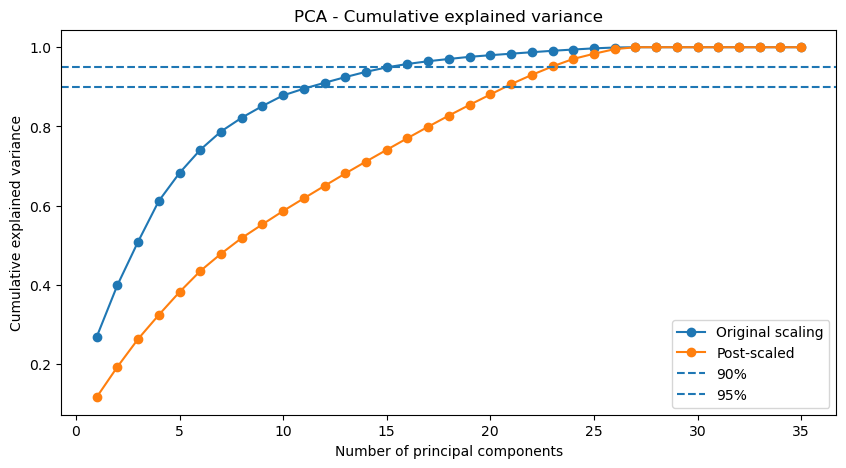
\includegraphics[width=.80\linewidth,height=.68\textheight,keepaspectratio]{plot_cell_60_1.png}
\keypoint{Per la stessa frazione di varianza, il numero di componenti dipende sensibilmente dallo scaling.}
\end{frame}

\begin{frame}{PCA: confronto quantitativo delle prestazioni}
\centering\small
\begingroup\renewcommand{\arraystretch}{1.05}
\begin{tabular}{@{}llrr@{}}\toprule
\textbf{Scaling} & \textbf{PCA} & \textbf{Componenti} & \textbf{CV AP}\\\midrule
Originale & No & 35 & 0,3550\\
Originale & 90\% & 12 & 0,2839\\
Originale & 95\% & 16 & 0,2849\\\midrule
Globale & No & 35 & 0,3548\\
\rowcolor{pale} Globale & 90\% & \textbf{21} & \textbf{0,3557}\\
Globale & 95\% & 23 & 0,3556\\\bottomrule\end{tabular}\endgroup
\par\vspace{.15em}
\begin{itemize}\setlength{\itemsep}{.1em}
\item PCA 90\% dopo scaling globale: \textbf{35 $\to$ 21} componenti, AP comparabile.
\item Nessun miglioramento predittivo sostanziale; interpretabilità ridotta.
\end{itemize}
\keypoint{Decisione finale: mantenere la rappresentazione originale.}
\source{Dimensioni misurate sul fit dell'intero training; durante la CV il numero può variare tra fold.}
\end{frame}

\begin{frame}{Esperimento diagnostico: reintrodurre \texttt{duration}}
\begin{columns}[c,onlytextwidth]
\column{.58\textwidth}
\centering
\begin{tabular}{@{}lr@{}}\toprule
\textbf{Logistic Regression} & \textbf{CV AP}\\\midrule
Senza \texttt{duration} & 0,3550\\
\rowcolor{pale} Con \texttt{duration} & \textbf{0,5199}\\\bottomrule\end{tabular}
\par\vspace{.95em}
{\Large\bfseries\color{teal} $+0,165$ AP}
\column{.39\textwidth}
\begin{block}{Interpretazione}
La feature è estremamente informativa, ma \textbf{non disponibile prima del contatto}.
\end{block}
\vspace{.5em}
{\small Esperimento separato; non modifica il prediction setting del modello finale.}
\end{columns}
\end{frame}

\section{Decisione e valutazione}

\begin{frame}{Threshold tuning: dagli score alla classe}
\begin{columns}[T,onlytextwidth]
\column{.54\textwidth}
\textbf{Modello selezionato}: tuned Random Forest, secondo la CV AP.
\vspace{.6em}
\begin{itemize}\tightitems
\item Generazione di score \textbf{out-of-fold} sul training.
\item Valutazione di soglie candidate ricavate dagli score.
\item Selezione della soglia che massimizza $F_1$.
\end{itemize}
\[\tau^*=\arg\max_{\tau}F_1(\tau)\]
\column{.42\textwidth}
\begin{block}{Risultato OOF}
\centering
{\LARGE\bfseries\color{teal}$\tau^*=0,1913$}\par\smallskip
\begin{tabular}{@{}lr@{}}Precision & 0,4103\\Recall & 0,4077\\F1 & 0,4090\end{tabular}
\end{block}
\end{columns}
\source{F1 è un compromesso convenzionale, poiché non è disponibile una matrice di costi e benefici.}
\end{frame}

\begin{frame}{Threshold tuning: Precision, Recall e F1}
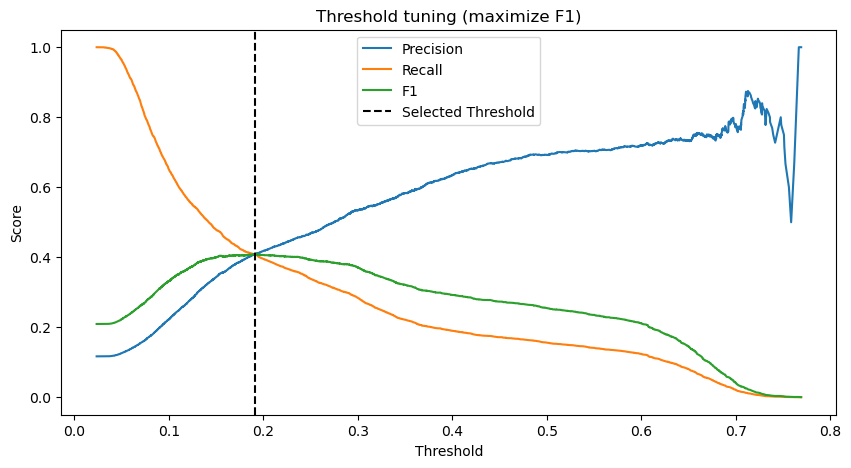
\includegraphics[width=.82\linewidth,height=.70\textheight,keepaspectratio]{plot_cell_64_1.png}
\keypoint{La soglia selezionata ($\approx0,191$) è inferiore a quella di default (0,5).}
\end{frame}

\begin{frame}{Valutazione finale: tuned Random Forest sul test}
\begin{columns}[T,onlytextwidth]
\column{.49\textwidth}
\textbf{Metriche sul test}\par\medskip
\begin{tabular}{@{}lr@{}}\toprule
Accuracy & 0,8644\\
Precision & 0,4200\\
Recall & 0,4168\\
F1 & 0,4184\\
ROC-AUC & 0,7497\\
\rowcolor{pale} \textbf{Average Precision} & \textbf{0,3909}\\\bottomrule\end{tabular}
\column{.46\textwidth}
\begin{block}{Confronto AP}
\centering
\begin{tabular}{@{}lr@{}}CV sul train & 0,3841\\Test finale & \textbf{0,3909}\end{tabular}
\end{block}
\vspace{.6em}
{\small L'AP sul test è vicina a quella stimata in CV: non emerge un peggioramento evidente del ranking sul campione di test.}
\end{columns}
\end{frame}

\begin{frame}{Curva Precision--Recall sul test}
\begin{columns}[c,onlytextwidth]
\column{.65\textwidth}
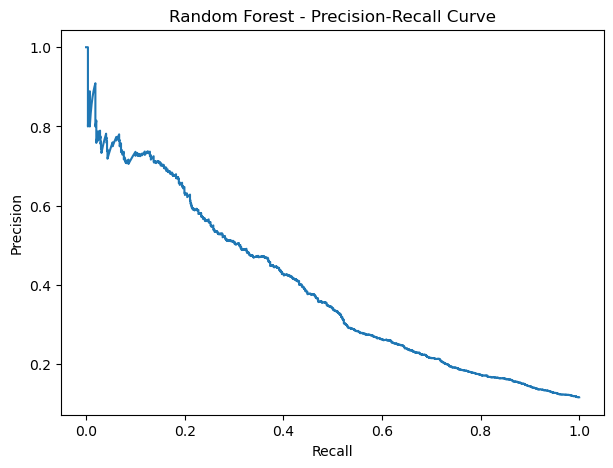
\includegraphics[width=\linewidth,height=.72\textheight,keepaspectratio]{plot_cell_66_1.png}
\column{.31\textwidth}
\textbf{AP sul test}\par\medskip
{\LARGE\bfseries\color{teal}0,3909}\par\vspace{1.2em}
\textbf{Prevalenza positiva}\par\medskip
{\Large\bfseries 0,1170}\par\vspace{.7em}
{\small Il ranking concentra i veri positivi più di una scelta casuale.}
\end{columns}
\end{frame}

\begin{frame}{Confusion matrix e compromesso operativo}
\begin{columns}[c,onlytextwidth]
\column{.55\textwidth}
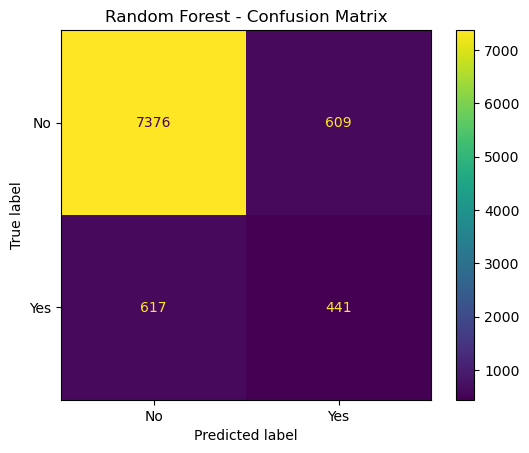
\includegraphics[width=\linewidth,height=.69\textheight,keepaspectratio]{plot_cell_67_0.png}
\column{.42\textwidth}
\begin{tabular}{@{}lr@{}}\toprule
True Positive & \textbf{441}\\
False Positive & 609\\
False Negative & 617\\
True Negative & 7.376\\\bottomrule\end{tabular}
\par\vspace{.75em}
{\small\noindent\parbox{\linewidth}{La soglia selezionata recupera parte dei positivi, accettando falsi positivi. L'Accuracy può essere inferiore a quella della baseline sempre negativa.}}
\end{columns}
\end{frame}

\begin{frame}{Interpretazione operativa: prioritizzazione}
\centering
\begin{tabular}{@{}lr@{}}\toprule
Clienti nel test & 9.043\\
Clienti classificati positivi & \textbf{1.050}\\
Sottoscrittori tra i classificati positivi & \textbf{441}\\
Precision del gruppo selezionato & \textbf{42,0\%}\\
Prevalenza generale & 11,7\%\\\bottomrule\end{tabular}
\par\vspace{.95em}
{\normalsize\bfseries\color{teal} Concentrazione dei positivi $\approx 3,6\times$ la prevalenza generale}\par
\vspace{.75em}
\begin{block}{Attenzione}
Questo risultato illustra l'utilità del \textbf{ranking}; non costituisce una misura di profitto senza costi, ricavi e budget della campagna.
\end{block}
\end{frame}

\section{Error Analysis}

\begin{frame}{Error analysis: storico dei contatti}
\centering
\begin{tabular}{@{}lrrrr@{}}\toprule
\textbf{\texttt{prev\_cont}} & \textbf{Support} & \textbf{Positivi reali} & \textbf{Recall} & \textbf{FNR}\\\midrule
\texttt{0} & 7.370 & 657 & 18,57\% & 81,43\%\\
\rowcolor{pale}\texttt{1} & 1.673 & 401 & 79,55\% & 20,45\%\\\bottomrule
\end{tabular}
\par\vspace{1em}
\begin{itemize}\setlength{\itemsep}{.7em}
\item Il Recall cresce da \textbf{18,57\%} a \textbf{79,55\%} nei clienti già contattati in campagne precedenti.
\item In assenza di uno storico informativo il modello tende a non riconoscere molti clienti che poi sottoscrivono.
\end{itemize}
\source{Analisi descrittiva sul test, non usata per modificare il modello.}
\end{frame}

\begin{frame}{Error analysis: \texttt{poutcome}}
\centering\small
\begin{tabular}{@{}lrrrrr@{}}\toprule
\textbf{Esito precedente} & \textbf{Support} & \textbf{Positivi reali} & \textbf{Recall} & \textbf{FNR} & \textbf{FPR}\\\midrule
\texttt{unknown} & 7.370 & 657 & 18,57\% & 81,43\% & 3,46\%\\
\texttt{failure} & 1.012 & 140 & 56,43\% & 43,57\% & 22,13\%\\
\texttt{other} & 355 & 62 & 66,13\% & 33,87\% & 26,28\%\\
\rowcolor{pale}\texttt{success} & 306 & 199 & 100\% & 0\% & 100\%\\\bottomrule
\end{tabular}
\par\vspace{.9em}
\begin{itemize}\setlength{\itemsep}{.6em}
\item Nel test, \texttt{poutcome=unknown} identifica lo stesso gruppo di \texttt{prev\_cont=0}: non sono due evidenze indipendenti.
\item Con \texttt{poutcome=success}, tutti i 306 clienti del gruppo vengono classificati positivi alla soglia fissata, inclusi i 107 negativi reali.
\end{itemize}
\source{Risultati specifici del campione di test; non rappresentano regole universali.}
\end{frame}

\begin{frame}{Error analysis: \texttt{housing} e \texttt{loan}}
\centering
\begin{tabular}{@{}lrr@{}}\toprule
\textbf{Sottogruppo} & \textbf{Recall} & \textbf{FNR}\\\midrule
\texttt{housing=yes} & 16,62\% & 83,38\%\\
\texttt{housing=no} & 55,67\% & 44,33\%\\\midrule
\texttt{loan=yes} & 13,64\% & 86,36\%\\
\texttt{loan=no} & 44,23\% & 55,77\%\\\bottomrule\end{tabular}
\vspace{1.1em}
\keypoint{I gruppi associati a tassi di sottoscrizione inferiori nell'EDA presentano anche più positivi non riconosciuti.}
\vspace{.45em}
{\small I tassi sono condizionati al gruppo; non implicano relazioni causali.}
\end{frame}

\begin{frame}{Error analysis: differenze tra categorie professionali}
\centering\small
\begin{tabular}{@{}lrrr@{}}\toprule
\textbf{Job} & \textbf{Positivi nel gruppo} & \textbf{Recall} & \textbf{FPR}\\\midrule
Student & 50 & 84,00\% & 61,54\%\\
Retired & 100 & 78,00\% & 34,38\%\\
Blue-collar & 137 & 24,09\% & 1,87\%\\
Entrepreneur & 22 & 9,09\% & 2,15\%\\\bottomrule\end{tabular}
\vspace{1em}
\begin{itemize}\tightitems
\item Alcuni gruppi ricevono frequentemente predizioni positive: Recall elevato \emph{e} FPR elevato.
\item Interpretare con prudenza le categorie con pochi esempi positivi (es. \texttt{entrepreneur}).
\end{itemize}
\end{frame}

\begin{frame}{Error analysis: distribuzione degli score}
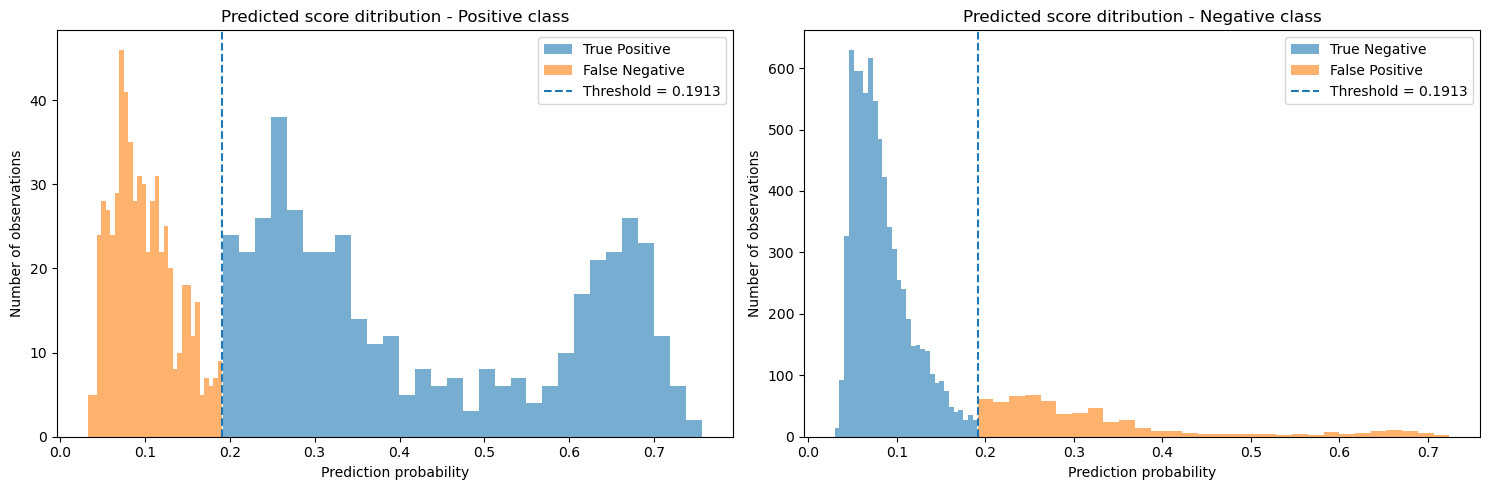
\includegraphics[width=.91\linewidth,height=.67\textheight,keepaspectratio]{plot_cell_74_0.png}
\keypoint{False positive: score alti senza sottoscrizione. False negative: positivi reali con score sotto la soglia.}
\end{frame}

\begin{frame}{Confident errors: due pattern ricorrenti}
\begin{columns}[T,onlytextwidth]
\column{.48\textwidth}
\begin{block}{False positive con score più alti}
\begin{itemize}\tightitems
\item \texttt{poutcome=success}
\item \texttt{prev\_cont=1}
\item Frequentemente \texttt{housing=no}, \texttt{loan=no}
\end{itemize}
\end{block}
\column{.48\textwidth}
\begin{block}{False negative con score più bassi}
\begin{itemize}\tightitems
\item Frequentemente \texttt{poutcome=unknown}
\item \texttt{prev\_cont=0}
\item Spesso \texttt{housing=yes} e \texttt{blue-collar}
\end{itemize}
\end{block}
\end{columns}
\vspace{.8em}
\keypoint{L'assenza di una storia precedente informativa è associata a maggiori difficoltà nel riconoscere i positivi.}
\end{frame}

\section{Conclusioni}

\begin{frame}{Limitations: validità del contesto e delle informazioni}
\begin{itemize}\setlength{\itemsep}{1.05em}
\item \textbf{Dati storici}: uno split casuale stratificato non sostituisce una validazione su campagne temporalmente successive.
\item \textbf{Prediction setting}: la disponibilità di \texttt{contact}, \texttt{day}, \texttt{month}, \texttt{duration} dipende dallo scenario operativo.
\item \textbf{Storico aggregato}: \texttt{pdays}, \texttt{previous}, \texttt{poutcome} non costituiscono una cronologia completa delle interazioni.
\item \textbf{Associazioni, non causalità}: EDA ed error analysis non misurano effetti causali.
\end{itemize}
\end{frame}

\begin{frame}{Limitations: soglia e utilizzo operativo}
\begin{block}{Soglia scelta sul training}
\vspace{.2em}
La soglia $\tau^*\approx0,1913$ massimizza l'F1 sulle predizioni out-of-fold. Senza informazioni sui costi e sui benefici, non possiamo considerarla \textbf{economicamente ottimale}.
\end{block}
\vspace{.75em}
\textbf{Prima di un'applicazione reale servirebbero:}
\begin{itemize}\setlength{\itemsep}{.6em}
\item una validazione su campagne temporalmente successive;
\item una stima del costo dei contatti e del beneficio delle sottoscrizioni;
\item la definizione di un budget e di una soglia decisionale coerente con gli obiettivi della campagna.
\end{itemize}
\end{frame}

\begin{frame}{Conclusioni principali}
\begin{enumerate}\setlength{\itemsep}{1em}
\item Il \textbf{prediction setting} guida la scelta delle variabili: \texttt{duration} è predittiva ma esclusa.
\item La \textbf{Random Forest ottimizzata} è il miglior modello per AP fra quelli confrontati (CV $0,3841$; test $0,3909$).
\item La \textbf{regolarizzazione degli alberi} riduce marcatamente l'overfitting iniziale.
\item \textbf{Feature selection e PCA} comprimono i dati, ma non migliorano sostanzialmente l'AP.
\item L'\textbf{error analysis} rivela una forte dipendenza dalle informazioni sui contatti precedenti.
\end{enumerate}
\vspace{.35em}
\keypoint{Il modello è promettente per prioritizzare i clienti, previa validazione operativa e temporale.}
\end{frame}

\begin{frame}[standout]
Grazie per l'attenzione
\end{frame}

\appendix
\begin{frame}{Appendice: metriche e threshold}
\small
\begin{tabular}{@{}ll@{}}\toprule
Metrica & Interpretazione\\\midrule
Precision & $TP/(TP+FP)$\\
Recall & $TP/(TP+FN)$\\
F1 & $2\cdot\mathrm{Precision}\cdot\mathrm{Recall}/(\mathrm{Precision}+\mathrm{Recall})$\\
FPR & $FP/(FP+TN)$\\
FNR & $FN/(TP+FN)$\\\bottomrule\end{tabular}
\par\vspace{1em}
{\small La baseline sempre negativa ha accuracy $\approx88,3\%$, ma Recall e F1 della classe positiva pari a zero.}
\end{frame}
\begin{frame}{Appendice: condizioni per la feature selection}
\begin{itemize}\setlength{\itemsep}{1em}
\item Le 35 \emph{feature} si riferiscono alle \textbf{colonne dopo lo scaling/one-hot encoding}, non alle 16 variabili originali.
\item Le feature riportate come selezionate sono ottenute dal fit del selettore sull'intero training set.
\item Nella CV, \texttt{SelectFromModel} e PCA sono \textbf{rifittati dentro ogni fold}: le feature e il numero di componenti possono cambiare.
\item Ridurre la dimensionalità non garantisce un miglioramento predittivo.
\end{itemize}
\end{frame}
\end{document}
